%%%%%%%%%%%%%%%%%%%%%%%%%%% Figure 3 Godafoss %%%%%%%%%%%%%%%%%%%%%%%%%%%%%%%
\begin{figure}[t]
 \begin{center}
  \begin{pspicture}(0,0)(15,10)
% Include graphs
   \rput[b](7.7, 0.0){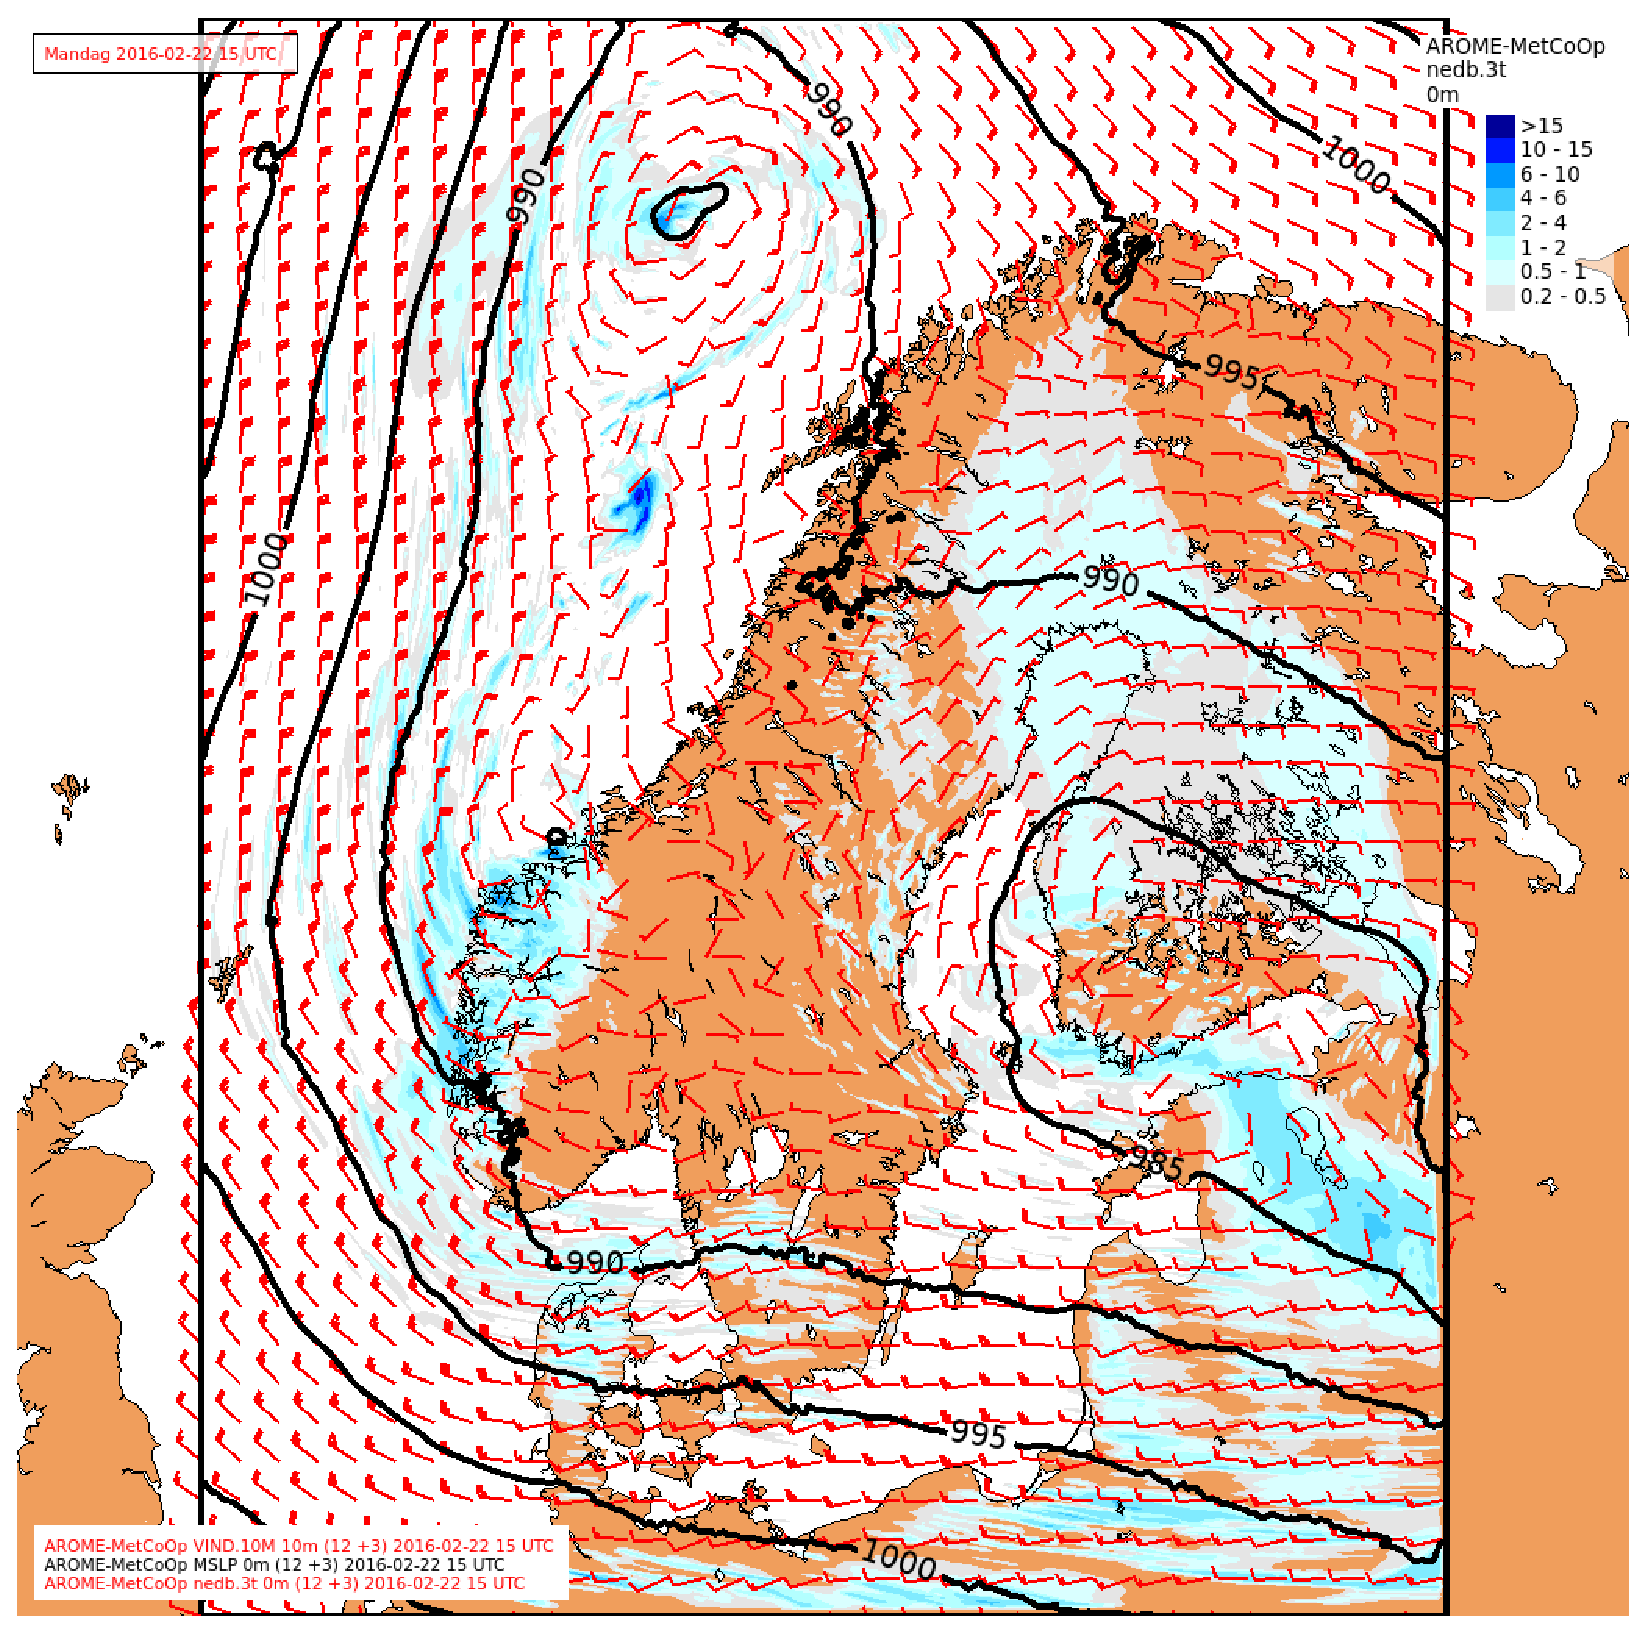
\includegraphics[height=10cm]{AROME_2016-02-22_15UTC}}
  \end{pspicture}
  \caption{\small The area covered by the Arome-MetCoop model. Shown is the forecasted (lead time 3 hrs) mean sea level pressure in hPa (black solid lines, countour interval = 5 hPa), 3 hourly precipitation, and 10 m wind valid at 1500UTC on February 22, 2016. Color bar indicates precipitation with a variable contour interval in the range 0.2-15 mm or larger (deep blue).} 
  \label{fig:arome}
 \end{center}
\end{figure}

